\documentclass[journal]{IEEE_JAIC}


\usepackage[serbian]{babel}


\usepackage[pdftex]{graphicx}

\usepackage{tikz}

% Required packages by the template
\usepackage{xcolor}
\usepackage[utf8]{inputenc}

\title{Iks-oks igra sa umjetnom inteligencijom \\
    \large Projekat za Praktikum elektronike \\
    Profesor: red. prof. dr Abdulah Akšamović}
\author{Student: Berina Biberović \\
        Univerzitet u Sarajevu, Elektrotehnički fakultet, Sarajevo, Bosna i Hercegovina \\
        bbiberovic1@etf.unsa.ba}
%\professor{Red. prof. dr Abdulah Akšamović}
        
% Logo image
\usepackage{eso-pic}
\AddToShipoutPictureBG*{%
    \AtPageUpperLeft{\put(100, -190){
\includegraphics[width=0.2\textwidth]{Slike/unsa.jpg}}
    }
}


\newcommand{\placetextbox}[3]{
    \setbox0=\hbox{#3}
    \AddToShipoutPictureFG{ \put(\LenToUnit{#1\paperwidth},\LenToUnit{#2\paperheight}){\vtop{{\null}\makebox[0pt][c]{#3}}}
    }
}


\begin{document}


{\maketitle}

\begin{tikzpicture}[remember picture,overlay]
   \node[anchor=north east,inner sep=3cm] at (current page.north east)
              {
\includegraphics[width=0.2\textwidth]{Slike/ETF_logo.png}};
\end{tikzpicture}



\begin{abstract}
U ovom radu je prikazana iks-oks igra (engl. tic-tac-toe) implementirana uz pomoć PIC16F1939 mikrokontrolera. Implementirano je rješenje koje omogućava da dva igrača igraju igru ili da igrač igra protiv mašine. Prikaz stanja igre je urađen preko mreže svijetlećih dioda. Multipleksiranjem izlaza mikrokontrolera pomoću prekida je omogućeno prikazivanje trenutnog stanja table. U prilogu je pokazan i PCB razvoj ovog sistema koji je urađen u \textit{Proteus} okruženju. Objašnjava se detaljnije implementacija odgovarajućeg algoritma za umjetnu inteligenciju koji nije savršen, te neuspjela implementacija savršenog algoritma za umjetnu inteligenciju koji bi uvijek završavao pobjedom ili neriješenim rezultatom. Algoritam je rađen u \textit{MPLAB X} razvojnom paketu sa XC8 kompajlerom.
\end{abstract}


\section{Uvod}

Iks-oks je jednostavna igra pune informacije za dva igrača. Igra se na kvadratnoj tabli sa $3$ reda i $3$ kolone jednakih kvadratnih polja. Igrači alterniraju poteze. Prvi igrač na proizvoljno prazno polje postavi svoj znak X, odnosno "iks." $\,$ Nakon toga, drugi igrač na prazno polje postavlja O ili "oks," $\,$ nakon čega ponovo igra prvi igrač i procedura se ponavlja. \\

Igra završava pobjedom jednog od igrača ukoliko popuni jedan red, jednu kolonu ili jednu dijagonalu table isključivo sa svojim znakovima (dakle znakovima X u slučaju prvog igrača ili O u slučaju drugog igrača). Ukoliko se svih 9 polja popuni bez pobjede ijednog igrača igra se završava neriješenim rezultatom. \\

Ova igra je izučavana i riješena je, što znači da je poznat matematički optimalan pristup igranju. U slučaju da oba igrača igraju optimalno, igra će se uvijek završiti izjednačenim rezultatom. \\

Na slici \ref{fig:optigra} je predstavljen grafički prikaz optimalne strategije prvog igrača koja garantuje da će prvi igrač uvijek pobijediti ili izjednačiti, neovisno od strategije drugog igrača. Svojom optimalnom strategijom, drugi igrač može uvijek osigurati za sebe pobjedu ili nerješen rezultat, u ovisnosti od poteza koje prvi igrač odigra.\\

\begin{figure}
    \centering
    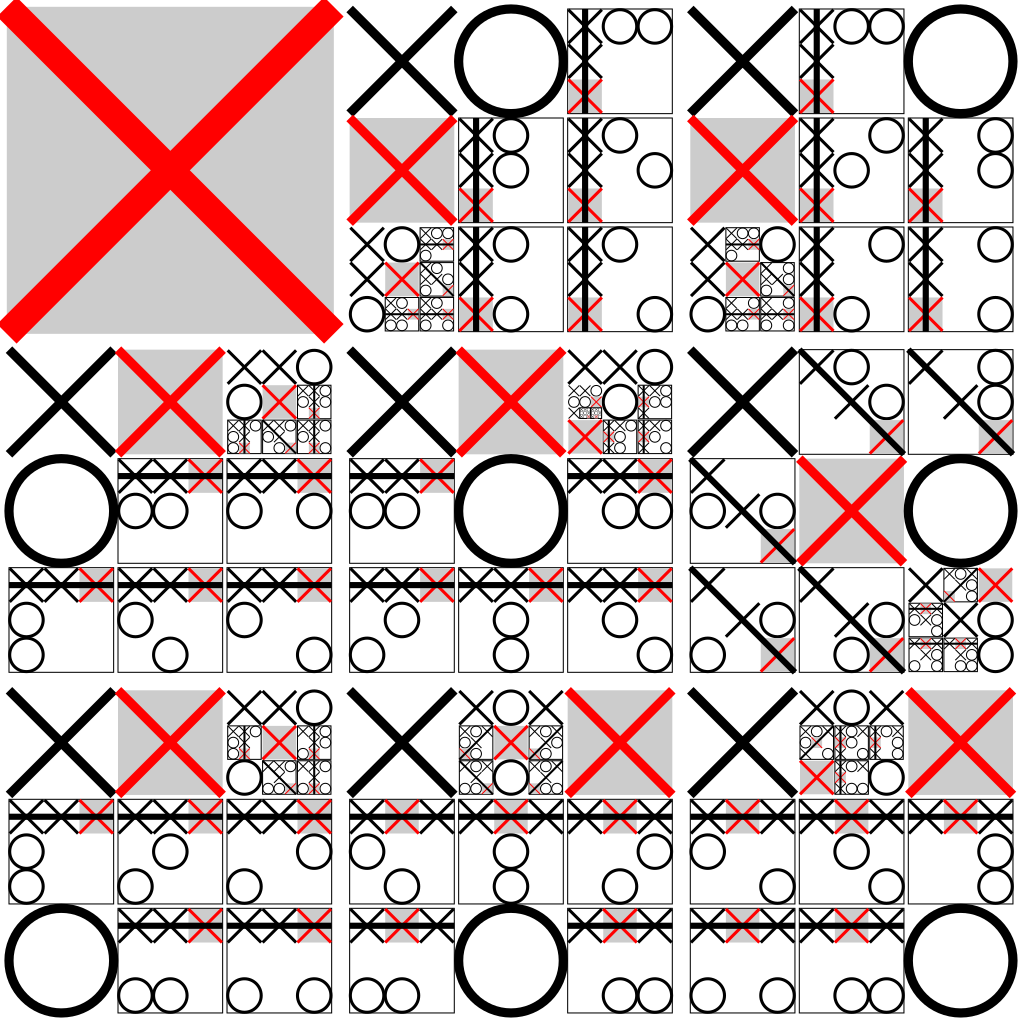
\includegraphics[width = 0.8\linewidth]{Slike/1024px-Tictactoe-X.svg.png}
    \caption{Grafički prikaz optimalne strategije za prvog igrača\cite{slika1}}
    \label{fig:optigra}
\end{figure}

% Optimal decision tree for player X in Tic-Tac-Toe. Based on "A Fractal Guide to Tic Tac Toe" by Ian Stewart on August 1, 2000 Scientific American

U ovom radu, na način prikazan ispod, implementirana je iks-oks igra na mikrokontroleru PIC16F1939, koja omogućava korisnicima da međusobno igraju ovu igru, onemogućujući im da vrše nedozvoljene poteze kao što je postavljanje više od jednog znaka na svom potezu ili postavljanje znaka nakon završene igre.\\

Također je implementiran režim rada u kojem korisnik može igrati protiv mašine, odnosno umjetne inteligencije koja je implementirana na mikrokontroleru, za koju smatramo da igra na nivou uporedivom čovjeku koji ne poznaje optimalnu strategjiu.\\

\section{Implementacija}

\subsection{Hardver}

Shema implementacije rješenja iks-oks problema koji je opisan u uvodu je postavljena u potpoglavlju \textit{Dodaci} zajedno sa PCB shemom i shemama rasporeda komponenti na PCB pločici. \\

Način na koji je prikazana tablica je preko mreže $3\times3$ para LEDica - gdje je jedna ledica crvene a druga zelene boje, što predstavlja X, odnosno O. LEDice su povezane tako da je anoda jedne spojena na katodu druge LEDice i obratno. Jedan kraj tako spojenog para je povezan na odgovarajući pin na mikrokontroleru koji kontroliše koja će se LEDica upaliti (u zavisnosti od toga da li se prikazuje X ili O), dok drugi kraj je spojen na zajednički pin za svih devet parova LEDica koji alternira svoj naponski nivo, kako bi u odgovarajućim trenucima crvene ili zelene LEDice mogle biti upaljene. Pored toga su dodani otpornici na izlaze iz pinova mikrokontrolera kako LEDice ne bi pregorile. \\

U potpoglavlju \textit{Softver} je opisano na koji način je postignuto da nema zabune koja polja su slobodna u toku igre, a koja su zauzeta sa odgovarajućim znakom. \\

Unos odgovarajućeg znaka, bilo da se radi o igri igrač protiv igrača ili igrač protiv umjetne inteligencije, se vrši preko $3\times3$ mreže tzv. \textit{slide switch}-eva. Konkretno, u PCB shemi je modeliran model MMS1208 \textit{slide switch}-a, čiji PCB model je namjenski napravljen kao predložak u datoj shemi. Od korisnika se zahtjeva da unese odgovarajuću lokaciju svog znaka tako što izabere identičnu lokaciju na mreži \textit{switch}-eva, te onda pomjeri prekidač u jednu pa u drugu stranu. \\

Pored unosa odgovarajućeg znaka u mreži za igru, preko istih \textit{slide switch}-eva se pokreće i zaustavlja igra, bira za umjetnu inteligenciju da li igra prva ili druga (X ili O) te se bira način igre: igrač protiv igrača ili igrač protiv mašine. \\

Napajanje datog sistema je urađeno tako da se vanjski napon dovede na \textit{LM7805} naponski regulator, koji na svom izlazu daje napon od 5 V - napajanje $V_{dd}$ mikrokontrolera, dok je masa priključena na napajanje $V_{ss}$ mikrokontrolera. Pored toga, ostavljena je mogućnost da se dovede $V_{pp}$ napon na mikrokontroler, kao i spajanje programatora na mikrokontroler. \\

Važno je istaći ovdje dodatak odgovarajućih otpornika na mrežu sa \textit{switch}-evima; njihova jedina svrha je mogućnost da se uradi PCB dizajn datog sistema, jer inače se ne bi moglo pronaći rješenje koje bi povezalo sve komponente, a da vodovi ostanu na jednoj strani pločice. Dimenzija PCB pločice je $78 \; mm \times 108 \; mm$, i korištena je mogućnost da se sa obje strane pločice mogu montirati elementi. \\

\subsection{Softver}

Softver projekta je razvijen u \textit{MPLAB X} okruženju, koristeći \textit{XC8} kompajler. Ovaj kompajler omogućava razvoj na PIC16F1939 mikrokontroleru koristeći C programski jezik. \\

Kontrola LEDica kojima se prikazuje trenutno stanje table je izvršena multipleksiranjem izlaza mikrokontrolera pomoću tajmer prekida koji su hardverski podržani na mikrokontroleru. Svijetleće diode trepere frekvencijom od približno $30 \; Hz$, što smatramo da je dovoljno brzo kako bi ljudsko oko to interpretiralo kao konstantan rad dioda.\\

U toku izvršavanja jedne prekidne rutine, koja se aktivira približno svakih $16 \; ms$, stanje table se ažurira u skladu sa unesenim komandama od strane čovjeka, te se alternira boja dioda koja se u tom trenutku prikazuje. Zbog multipleksiranja u jednom trenutku se prikazuju samo sve aktivne zelene diode (iks) ili samo sve crvene diode (oks).\\

Kod je razvijen u skladu sa tehnikom funkcionalnog programiranja radi preglednosti i jednostavnosti koda. Dijelovi koda vezani za pojedinačne funkcionalnosti se lagano mogu promijeniti bez potrebe da se veliki dijelovi koda također promijene u skladu s tim.\\

Kod je pisan konsistentnim stilom koji uključuje pisanja imena funkcija sa velikim početnim slovom i varijabli sa malim početnim slovom, a kroz cijeli kod su pisani odgovarajući komentari za lakše razumjevanje i održavanje.\\

Pored dijela koda koji se bavi prekidima i prikazom stanja table, najnapredniji je dio za pravljenje odluke poteza računara, koji je u nastavku obrazložen. \\

Umjetna inteligencija sistema je implemenirana sa trostepenim pristupom. Prije svega, ukoliko umjetna inteligencija ili "mašina" $\,$ može pobijediti u idućem potezu, to će i uraditi. Drugo, ukoliko to nije slučaj, onda se provjerava da li ljudski igrač može u svom idućem potezu spojiti tri znaka zaredom i pobijediti. Ukoliko može, onda će računar to blokirati.\\

Posljednje, ukoliko nijedan igrač ne može pobijediti u jednom potezu znak se postavlja na prvo slobodno polje iz uređene liste polja. Prvo polje u toj listi je centralno polje, nakon kojeg idu dva susjedna polja na ivici van ćoškova, nakon čega su preferirana polja na ćoškovima prije preostalih polja na ivicama.\\

U našem testiranju ova trostepena strategija je pokazala dobre rezultate kao strategija koju nije prelagano pobijediti, ali koja nije savršena i koju nije nemoguće pobijediti. \\

Implementirana, ali ne i iskorištena je varijacija umjetne inteligencije koja igra na nižem nivou. Strategija se sastoji samo od uređene liste preferiranih polja. Ovo je u toku razvoja korišteno kao testna strategija za provjeru funkcionalnosti sistema, ali bi se dodatnim razvojem mogao iskoristiti za sistem sa podesivom izazovom koji nudi umjetna inteligencija.\\

Razvijena je i umjetna inteligencija sa savršenom strategijom, ali ona nije uključena u konačnu verziju rada. Ta umjetna inteligencija je koristila minimax pristup, koji efektivno simulira optimalnu strategiju protivnika i pobrine se da uvijek igra optimalan potez.\\

Ovaj algoritam je po svojoj prirodi rekurzivan i tako je i razvijen, implementiran i testiran, no problem je što kompajler XC8 ne podržava uopšte rekurziju \cite{xc8}. Razlog ovome je ograničenje mikrokontrolera koje ograničava pozive ugnježdenih funkcija na 14. Ovo ograničenje nije problematično za naš algoritam, pošto maksimalna dubina poziva je 10, ali kako se ne bi greškom prelazilo preko ovog ograničenja kompajler uopšte ne dopušta rekurziju.\\

Algoritam je moguće napraviti bez rekurzije, čak i bez ugnježdenih funkcija, ali smatramo da tako razvijen algoritam bi bio vrlo nepregledan, te da je bolje napraviti umjetnu inteligenciju sa drugim pristupom.

\section{Dodaci}

Na slici \ref{shema} je prikazana shema razvijenog sistema, dok na slikama \ref{sl1}, \ref{sl2}, \ref{sl3}, \ref{sl4} i \ref{sl5} su prikazani redom: PCB shema sistema, prikaz komponenti sistema sa gornje strane pločice, prikaz komponenti sistema sa donje strane pločice, 3D prikaz razvijenog sistema sa gornje strane pločice i 3D prikaz razvijenog sistema sa donje strane pločice. \\




\begin{figure}[h]
    \centering
    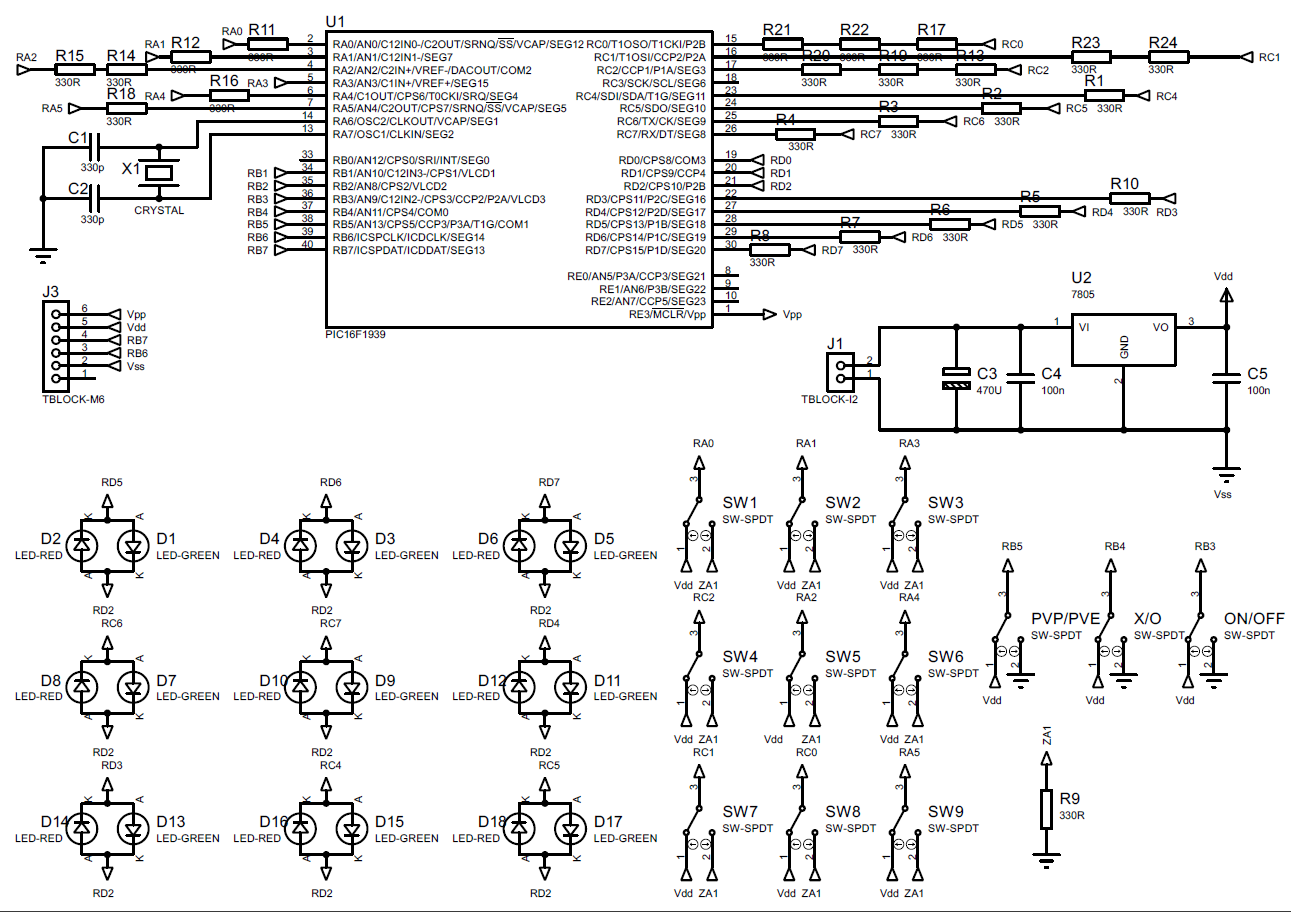
\includegraphics[width = 1\linewidth]{Slike/PE_Projekat_shema.png}
    \caption{Shema sistema}
    \label{shema}
\end{figure}

\begin{figure}[h]
    \centering
    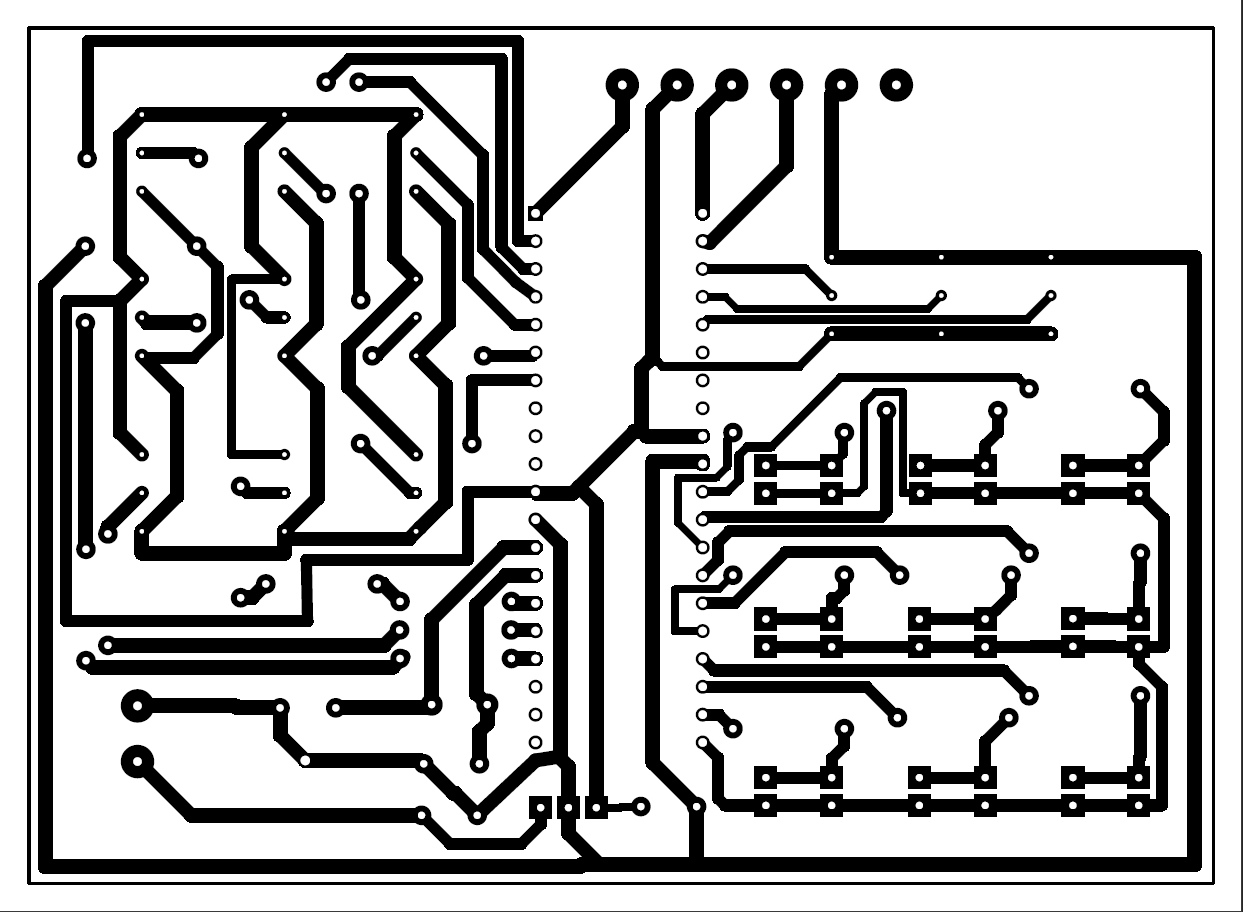
\includegraphics[width = 1\linewidth]{Slike/PE_Projekat_PCB.png}
    \caption{PCB shema sistema}
    \label{sl1}
\end{figure}

\begin{figure}[h]
    \centering
    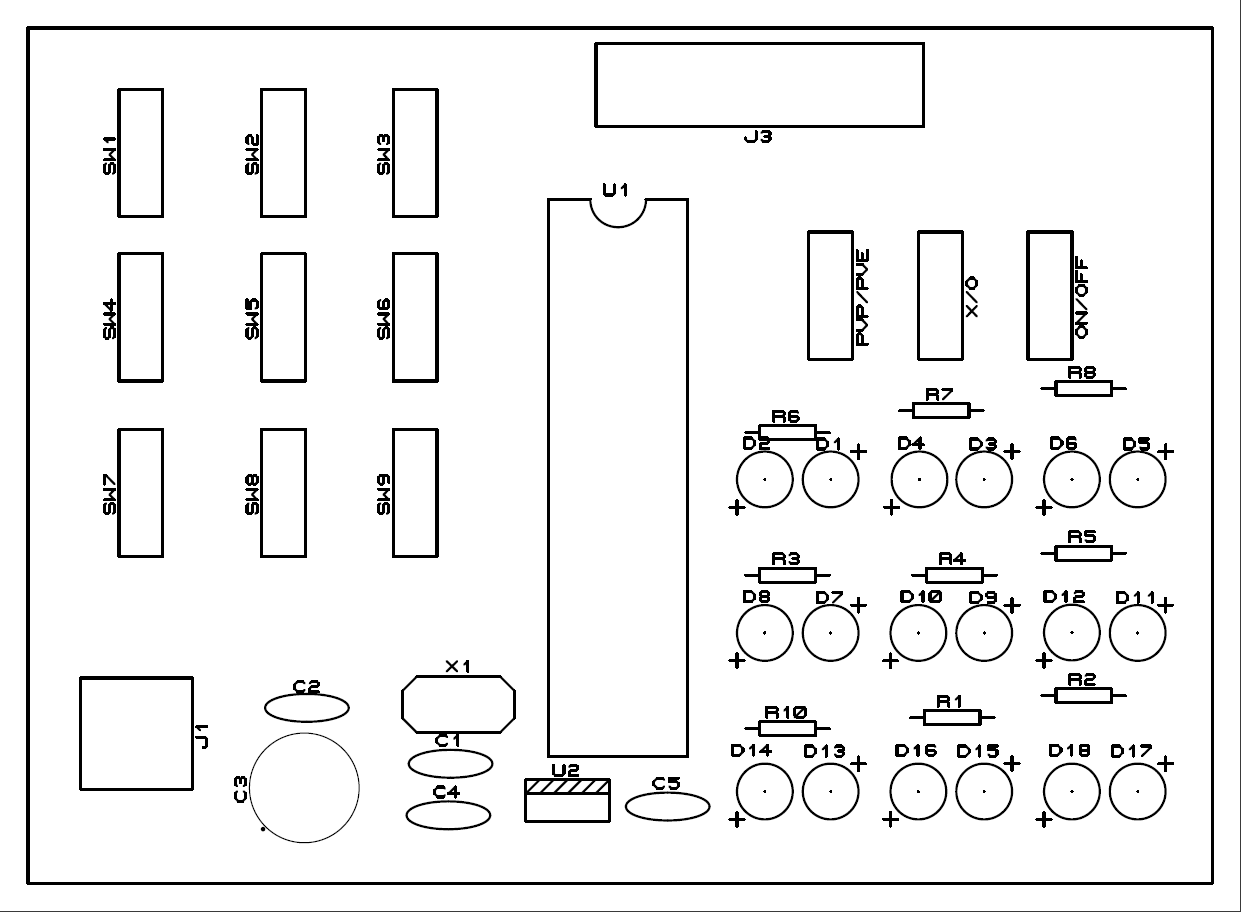
\includegraphics[width = 1\linewidth]{Slike/PE_Projekat_KOMPONENTE_GORE.png}
    \caption{Prikaz komponenti sa gornje strane}
    \label{sl2}
\end{figure}

\begin{figure}[h]
    \centering
    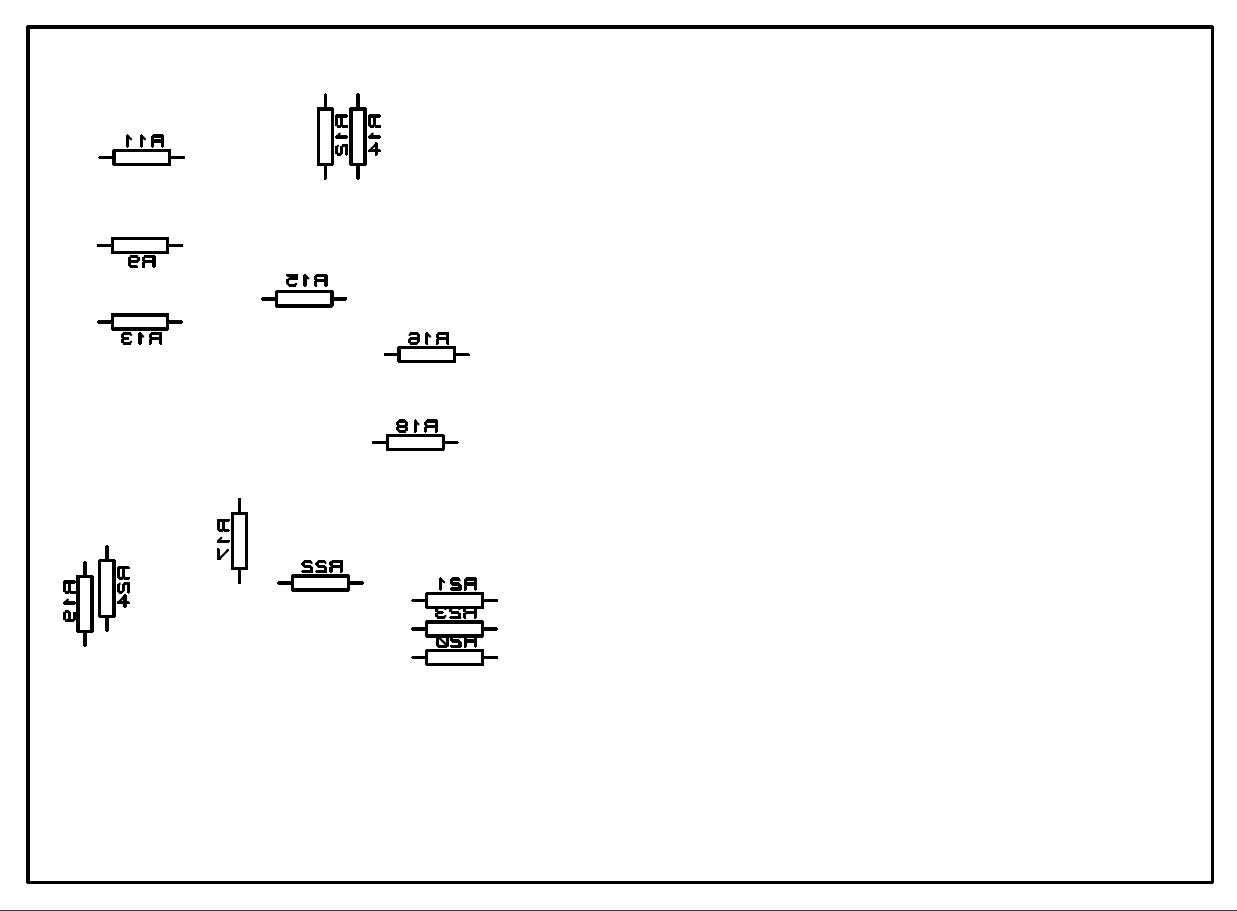
\includegraphics[width = 1\linewidth]{Slike/PE_Projekat_KOMPONENTE_DOLJE.png}
    \caption{Prikaz komponenti sa donje strane}
    \label{sl3}
\end{figure}

\begin{figure}[h]
    \centering
    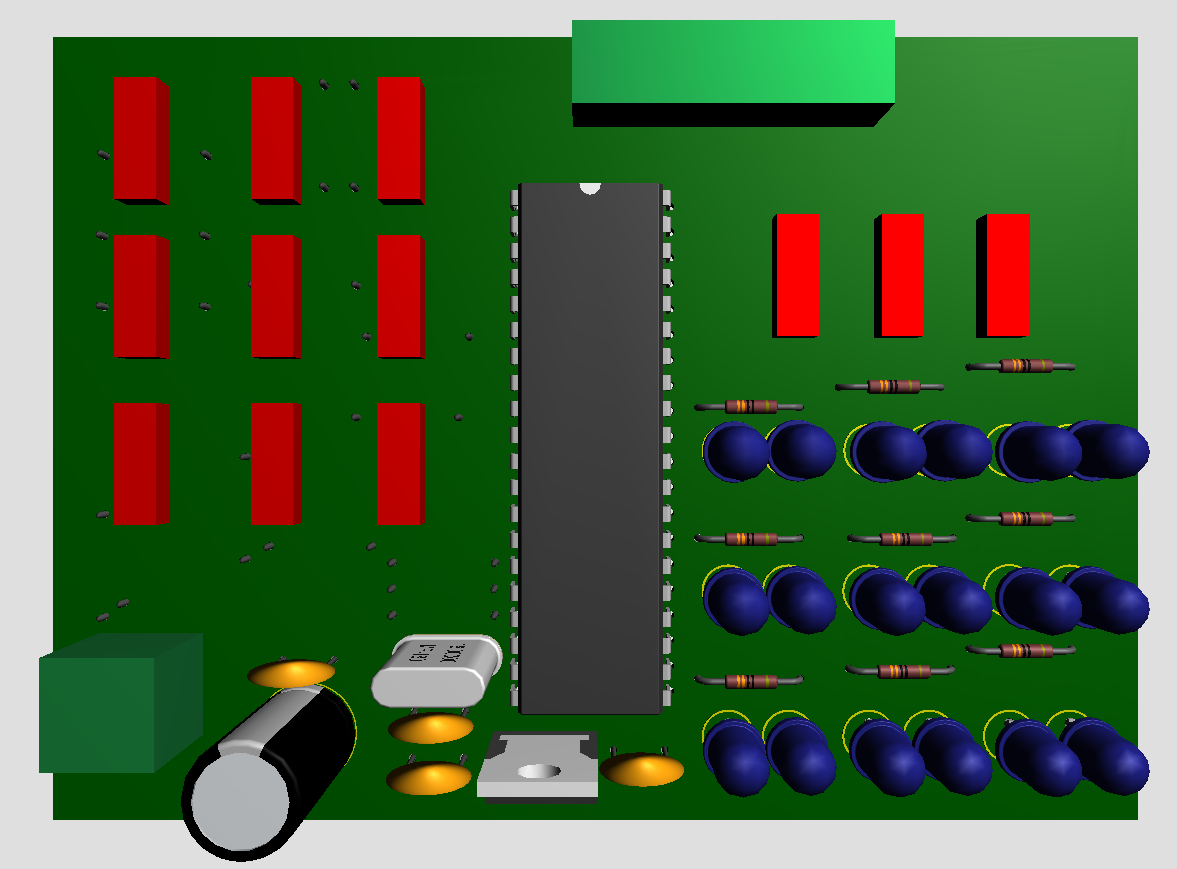
\includegraphics[width = 1\linewidth]{Slike/PE_Projekat_3D_GORE.png}
    \caption{3D prikaz sistema sa gornje strane}
    \label{sl4}
\end{figure}



\section{Zaključak}

PIC16F1939 je vrlo fleksibilan mikrokontroler. Sa oscilatorom od $8 \; MHz$ više je nego dovoljno brz za jednostavne igre i interakciju sa ljudima, a hardverski implementirana podrška za prekide preko timera mu omogućavaju multipleksiranu komunikaciju, čime koristi manje pinova od dikrektne izvedbe.\\

XC8 kompajler, podržan od strane razvojnog paketa \textit{MPLAB X} omogućava razvoj direktno u C programskom jeziku, što umnogome proširuje mogućnosti i olakšava razvoj na ovom mikrokontroleru. Ipak, primjetili smo da nije podržana potpuna kompatibilnost sa C programskim jezikom.\\

Ograničeni stek poziva funkcija onemogućava rekurziju dublju od 14 slojeva, a radi zaštite stabilnosti rada potpuno je onemogućeno rekurzivno pozivati funkcije koristeći XC8 kompajler.\\

Ipak, razvili smo efektivnu umjetnu inteligenciju za razumno kompetentno igranje ove jednostavne igre. \\

Razvili smo i PCB shemu koja sprema sistem za proizvodnju, uključujući interakciju sa čovjekom. Ukoliko bi se sistem proizvodio na većoj skali onda bismo predložili promjenu hardvera kako bi bila lakša interakcija između čovjeka i računara.\\

Veće pakovanje sa prekidačima koji su veći i lakši za koristiti bi umnogome poboljšalo iskustvo, no efektivno ne bi promjenilo funkcionalnost sistema. \\
\newline
\newline
\newline
\newline
\newline
\newline
\newline
\newline
\newline
\newline
\newline

\begin{figure}[h]
    \centering
    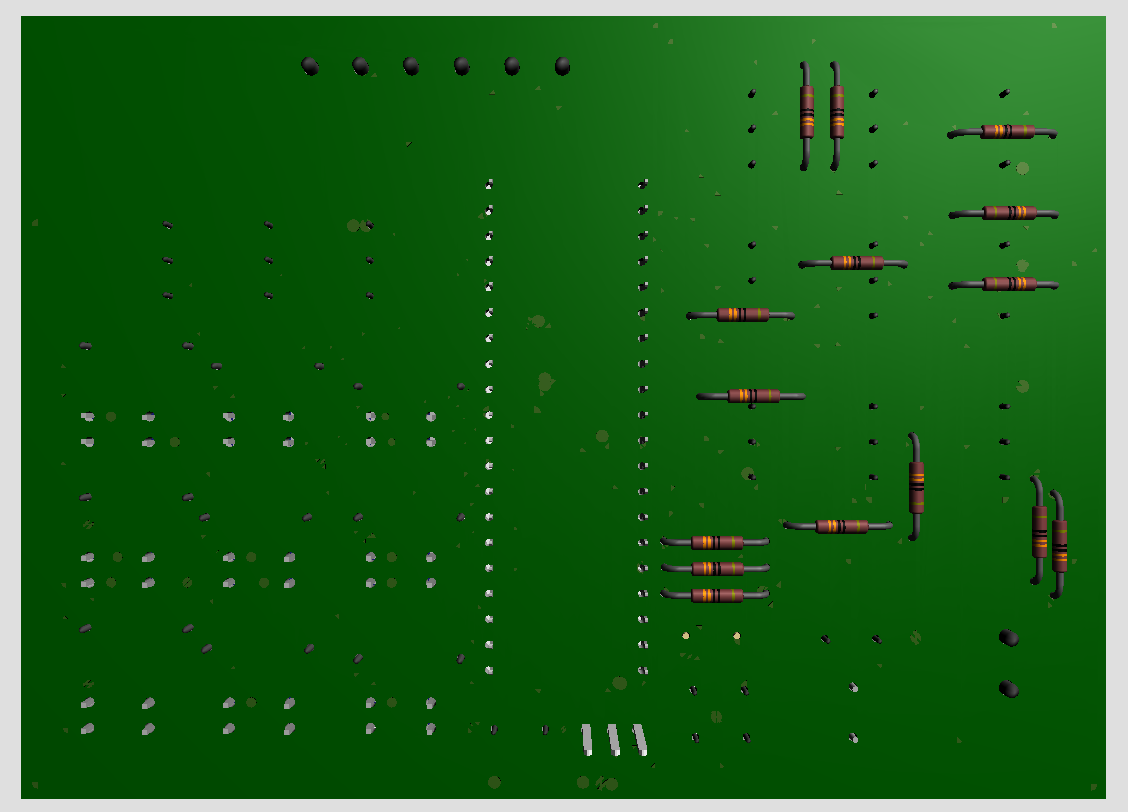
\includegraphics[width = 1\linewidth]{Slike/PE_Projekat_3D_DOLJE.png}
    \caption{3D prikaz sistema sa donje strane}
    \label{sl5}
\end{figure}


%ovdje ce ici literatura

\bibliographystyle{IEEEtran}
\bibliography{IEEEexample}






% that's all folks
\end{document}


